\subsection{使用深度 Q 网络解决推车杆问题}

在学习本节之前,可以先回顾一下之前的项目实战,即使用Q学习解决悬崖寻路问题。本节将具体实现深度 Q 网络算法来解决推车杆问题,对应的模拟环境为 OpenAI Gym 中的 CartPole-v0 ,我们同样先对该环境做一个简要说明。

\subsubsection{CartPole-v0 简介} 

CartPole-v0是一个经典的入门环境,如\figref{fig:cliffwalking} 所示,它通过向左(动作 = 0)或向右(动作 = 1)推动推车来实现推车杆的平衡。每次实施一个动作后,如果杆能够继续保持平衡,就会得到一个 $+1$ 的奖励,否则杆将无法保持平衡而导致游戏结束。理论上最优算法情况下,推车杆是能够一直保证平衡的,但是如果每回合无限制地进行下去,会影响到算法的训练,所以环境一般设置每回合的最大步数为200。另外 Gym 官方也推出了另外一版的推车杆环境,名为CartPole-v1,相比 v0 版本,v1每回合最大步数为500,其他基本不变,可以说是 v0 的难度升级版。

\begin{figure}[htb]
    \centering
    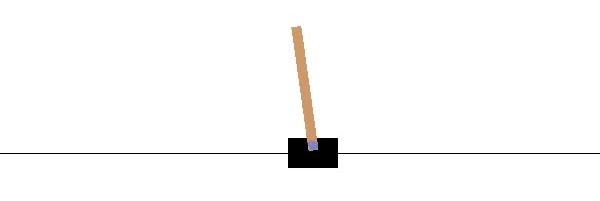
\includegraphics[width=0.6\linewidth]{res/ch7/assets/poster.jpg}
    \caption{CartPole-v0 环境}
    \label{fig:cliffwalking}
\end{figure}

我们来看看这个环境的一些参数,执行以下代码:

\begin{lstlisting}[style=Python]
    import gym
    env = gym.make('CartPole-v0')  # 建立环境
    env.seed(1) # 随机种子
    n_states = env.observation_space.shape[0] # 状态数
    n_actions = env.action_space.n # 动作数
    print(f"状态数:{n_states},动作数:{n_actions}")
\end{lstlisting}

可以得到结果:

\begin{lstlisting}[language=sh,basicstyle=\zihao{-5}\ttfamily] 
    状态数:4,动作数:2
\end{lstlisting}

该环境的状态数是4个,分别为车的位置、车的速度、杆的角度以及杆顶部的速度;动作数为2个,并且是离散的向左或者向右。

我们也可以直接重置或者初始化环境看看初始状态,代码如下:

\begin{lstlisting}[style=Python]
    state = env.reset() # 初始化环境
    print(f"初始状态:{state}")
\end{lstlisting}

结果为:

\begin{lstlisting}[language=sh,basicstyle=\zihao{-5}\ttfamily] 
    初始状态:[0.03073904  0.00145001 -0.03088818 -0.03131252]
\end{lstlisting}

\subsubsection{深度Q网络基本接口} 

介绍完环境之后,我们沿用接口的概念,通过分析伪代码来实现深度 Q 网络的基本训练模式。其实所有的强化学习算法都遵循同一个训练思路,执行动作,环境反馈,然后智能体更新,只是不同算法需要的一些要素不同,我们需要分析出这些要素,比如建立什么网络需要什么模块,以进一步完善算法。

我们现在常用的 深度Q网络 伪代码如\figref{fig:dqn} 所示。

\begin{figure}[htb]
    \centering
    
\includegraphics[width=0.75\linewidth]{res/ch7/assets/dqn.png}
    \caption{深度 Q 网络算法伪代码}
    \label{fig:dqn}
\end{figure}

用代码实现如下:

\begin{lstlisting}[style=Python]
    rewards = [] # 记录奖励
    ma_rewards = []  # 记录滑动平均奖励
    for i_ep in range(cfg.train_eps):
        state = env.reset() # 初始化环境
        done = False
        ep_reward = 0
        while True:
            action = agent.choose_action(state)
            next_state, reward, done, _ = env.step(action)
            ep_reward += reward
            agent.memory.push(state, action, reward, next_state, done)
            state = next_state
            agent.update()
            if done:
                break
        if (i_ep+1) % cfg.target_update == 0:
            agent.target_net.load_state_dict(agent.policy_net.state_dict())
        if (i_ep+1)%10 == 0:
            print('回合:{}/{}, 奖励:{}'.format(i_ep+1, cfg.train_eps, ep_reward))
        rewards.append(ep_reward)
        if ma_rewards:
            ma_rewards.append(0.9*ma_rewards[-1]+0.1*ep_reward)
        else:
            ma_rewards.append(ep_reward)
\end{lstlisting}

可以看到, 深度 Q 网络的训练模式其实和大多强化学习算法是一样的思路,但与传统的 Q 学习算法相比, 深度 Q 网络使用神经网络来代替之前的Q表格从而存储更多的信息,且由于使用了神经网络,因此我们一般需要利用随机梯度下降来优化 Q 值的预测。此外深度 Q 网络多了回放缓冲区,并且使用两个网络,即目标网络和当前网络。

\subsubsection{回放缓冲区} 

从伪代码中可以看出,回放缓冲区的功能有两个:一个是将每一步采集的经验(包括状态、动作、奖励、下一时刻的状态)存储到缓冲区中,并且缓冲区具有一定的容量(capacity);另一个是在更新策略的时候需要随机采样小批量的经验进行优化。因此我们可以定义一个 ReplayBuffer 类,包括 push() 和 sample() 两个函数,用于存储和采样。

\begin{lstlisting}[style=Python]
    import random
    class ReplayBuffer:
        def __init__(self, capacity):
            self.capacity = capacity # 回放缓冲区的容量
            self.buffer = [] # 缓冲区
            self.position = 0 
        
        def push(self, state, action, reward, next_state, done):
            ''' 缓冲区是一个队列,容量超出时删除开始存入的经验
            '''
            if len(self.buffer) < self.capacity:
                self.buffer.append(None)
            self.buffer[self.position] = (state, action, reward, next_state, done)
            self.position = (self.position + 1) % self.capacity 
        
        def sample(self, batch_size):
            batch = random.sample(self.buffer, batch_size) # 随机采小批量经验
            state, action, reward, next_state, done =  zip(*batch) # 解压成状态、动作等
            return state, action, reward, next_state, done
        def __len__(self):
            ''' 返回当前存储的量
            '''
            return len(self.buffer)
\end{lstlisting}

\subsubsection{ Q 网络} 

在深度 Q 网络中我们使用神经网络替代原有的Q表格,从而能够存储更多的Q值,实现更为高级的策略以便用于复杂的环境。这里我们用的是一个三层的感知机或者称之为连接网络:

\begin{lstlisting}[style=Python]
    class MLP(nn.Module):
        def __init__(self, input_dim,output_dim,hidden_dim=128):
            """ 初始化Q网络,为全连接神经网络
                input_dim: 输入的特征数即环境的状态数
                output_dim: 输出的动作维度
            """
            super(MLP, self).__init__()
            self.fc1 = nn.Linear(input_dim, hidden_dim) # 输入层
            self.fc2 = nn.Linear(hidden_dim,hidden_dim) # 隐藏层
            self.fc3 = nn.Linear(hidden_dim, output_dim) # 输出层
            
        def forward(self, x):
            # 各层对应的激活函数
            x = F.relu(self.fc1(x)) 
            x = F.relu(self.fc2(x))
            return self.fc3(x)
\end{lstlisting}

学过深度学习的读者应该对全连接神经网络十分熟悉。在强化学习中,网络的输入一般是状态,输出则是一个动作,假如总共有两个动作,那么这里的动作维度就是2,可能的输出就是0或1,一般我们用 ReLU 作为激活函数。根据实际需要也可以改变神经网络的模型结构等等,比如若我们使用图像作为输入,则可以使用卷积神经网络(convolutional neural network,CNN)。

\subsubsection{深度Q网络算法}

与前面的项目实战一样,深度 Q 算法一般也包括选择动作和更新策略两个函数,首先我们看选择动作:

\begin{lstlisting}[style=Python]
    def choose_action(self, state):
        '''选择动作
        '''
        self.frame_idx += 1
        if random.random() > self.epsilon(self.frame_idx):
            with torch.no_grad():
                state = torch.tensor([state], device=self.device, dtype=torch.float32)
                q_values = self.policy_net(state)
                action = q_values.max(1)[1].item() # 选择Q值最大的动作
        else:
            action = random.randrange(self.action_dim)
\end{lstlisting}

可以看到跟深度 Q 网络算法与 Q 学习算法其实是一样的,都是用的$\varepsilon$-贪心策略,只是深度 Q 网络算法我们需要通过 PyTorch 或者 TensorFlow 工具来处理相应的数据。

而深度 Q 网络算法更新策略的步骤稍微复杂一点儿,主要包括三个部分:随机采样、计算期望 Q 值和梯度下降,如下:

\begin{lstlisting}[style=Python]
    def update(self):
        if len(self.memory) < self.batch_size: # 当memory中不满足一个批量时,不更新策略
            return
        # 从回放缓冲区中随机采样一个批量的经验
        state_batch, action_batch, reward_batch, next_state_batch, done_batch = self.memory.sample(
            self.batch_size)
        # 转为张量
        state_batch = torch.tensor(state_batch, device=self.device, dtype=torch.float)
        action_batch = torch.tensor(action_batch, device=self.device).unsqueeze(1)  
        reward_batch = torch.tensor(reward_batch, device=self.device, dtype=torch.float)  
        next_state_batch = torch.tensor(next_state_batch, device=self.device, dtype=torch.float)
        done_batch = torch.tensor(np.float32(done_batch), device=self.device)
        
        q_values = self.policy_net(state_batch).gather(dim=1, index=action_batch) # 计算当前状态(s_t,a)对应的Q(s_t,a)
        next_q_values = self.target_net(next_state_batch).max(1)[0].detach() # 计算下一时刻的状态(s_t_,a)对应的Q值
        # 计算期望的Q值,对于终止状态,此时done_batch[0]=1, 对应的expected_q_values等于reward
        expected_q_values = reward_batch + self.gamma * next_q_values * (1-done_batch)
        loss = nn.MSELoss()(q_values, expected_q_values.unsqueeze(1))  # 计算均方根损失
        # 优化更新模型
        self.optimizer.zero_grad()  
        loss.backward()
        for param in self.policy_net.parameters():  # clip防止梯度爆炸
            param.grad.data.clamp_(-1, 1)
        self.optimizer.step() 
\end{lstlisting}

\subsubsection{结果分析}

实现代码之后,我们先来看看深度 Q 网络算法的训练效果,如\figref{fig:train_rewards_curve_cn-1689150.png} 所示。

\begin{figure}[htb]
    \centering
    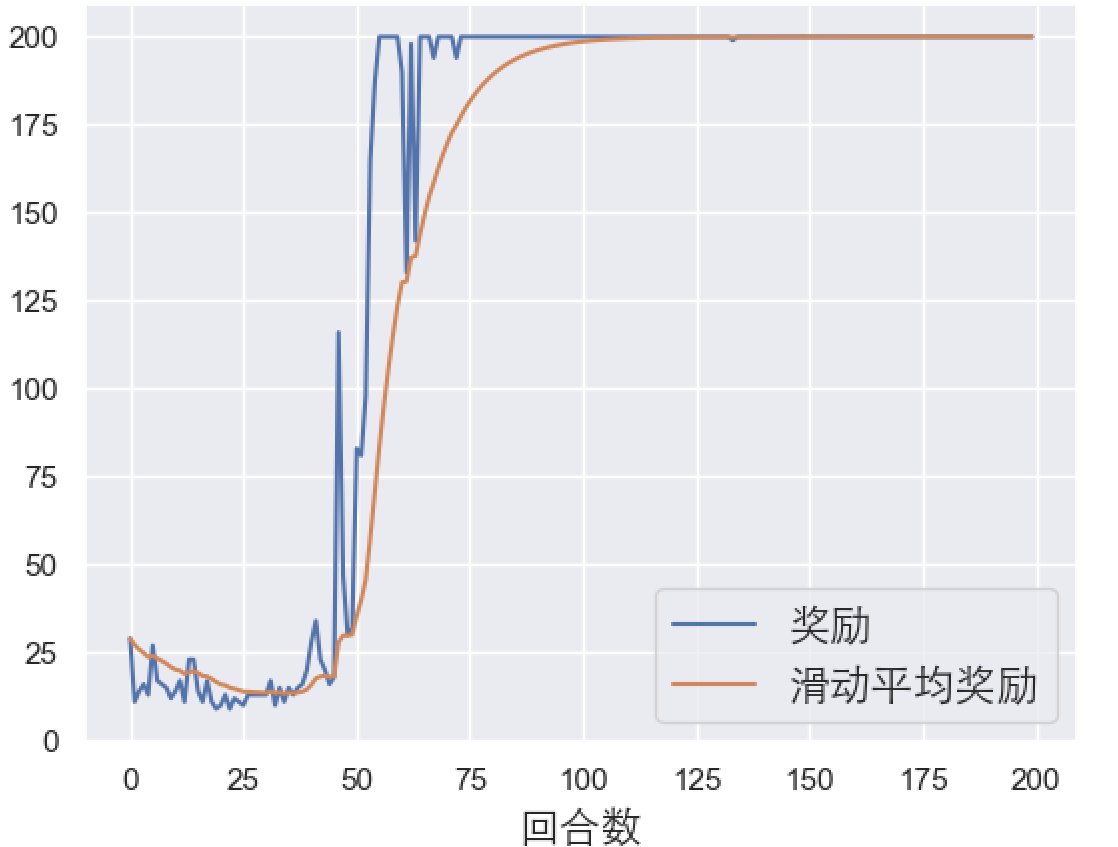
\includegraphics[width=0.6\linewidth]{res/ch7/assets/train_rewards_curve_cn-1689150.png}
    \caption{CartPole-v0 环境下深度 Q 网络算法的训练曲线}
    \label{fig:train_rewards_curve_cn-1689150.png}
\end{figure}

从\figref{fig:train_rewards_curve_cn-1689150.png} 中可以看出,算法其实已经在 60 回合左右达到收敛,最后一直维持在最佳奖励 200 左右,可能会有轻微的波动,这是因为我们在收敛的情况下依然保持了一定的探索率,即 epsilon\_end=0.01 。现在我们可以载入模型看看测试的效果,如\figref{fig:eval_rewards_curve_cn-1689282.png} 所示。

\begin{figure}[htb]
    \centering
    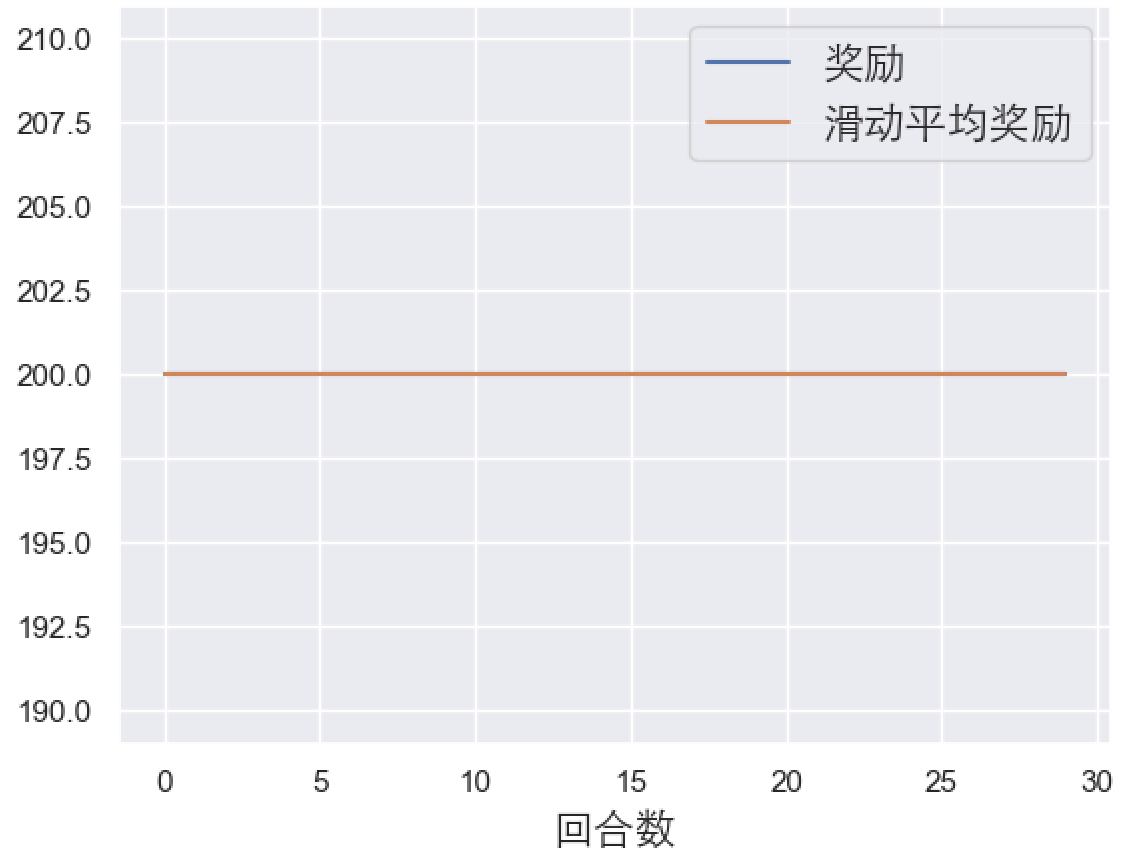
\includegraphics[width=0.6\linewidth]{res/ch7/assets/eval_rewards_curve_cn-1689282.png}
    \caption{CartPole-v0 环境下深度 Q 网络算法的测试曲线}
    \label{fig:eval_rewards_curve_cn-1689282.png}
\end{figure}

我们测试了 30 个回合,每个回合奖励都保持在 200 左右,说明我们的模型学习得不错!
